\documentclass[10pt,a4paper,titlepage]{article}
\usepackage[utf8]{inputenc}
\usepackage{amsmath}
\usepackage{amsfonts}
\usepackage{amssymb}
\usepackage{makeidx}
\usepackage{enumitem}
\usepackage{graphicx}
\usepackage{longtable}
\usepackage[hidelinks]{hyperref}

%this is a command used in the title template
\newcommand{\HRule}{\rule{\linewidth}{0.5mm}}

%questo fa in modo che le liste numerate siano allineate come le altre
\setenumerate{leftmargin=*, labelindent=\parindent}

%questo genera il toc, ricorda di eseguire due volte
\makeindex

\begin{document}
\begin{titlepage}
\begin{center}

%logo

\includegraphics[width=0.30\textwidth]{./images/logo}~\\[1cm]
\textsc{\LARGE Politecnico di Milano}\\[1.5cm]

\textsc{\Large Software Engineering 2 Project}\\[0.5cm]

% Title
\HRule \\[0.4cm]
{ \Huge \bfseries MeteoCal \\[0.4cm] }
{ \huge \bfseries Design Document \\[0.4cm] }
\HRule \\[1.5cm]

% Author
\begin{flushright}
\noindent
\large
\emph{Authors:}\\
Andrea \textsc{Celli}\\
Stefano \textsc{Cereda}
\end{flushright}
\vfill

% Bottom of the page
{\large \today}

\end{center}
\end{titlepage}

\part{Introduction}

\section{Purpose of this document}
This document describes the general and specific architecture of MeteoCal, the project of the course of Software Engineering 2 at Politecnico di Milano.
The document will explain the architectural decisions and trade offs chosen in the design process and its justifications.

\section{Scope}
The architectural descriptions provided concern the functional view, module view, deployment view, data layer, business logic and the user interface of the RASD.
Hence the architecture will consider the following functionalities offered by MeteoCal:

\begin{itemize}
\item \emph{Users:} MeteoCal will manage personal data of the users. MeteoCal will manage registering, logging in/out and the modification of personal data.

\item \emph{Calendars:} MeteoCal will manage a calendar for each user. User will be able to create, update and delete an event and to see other people's events. MeteoCal will also manage event invitation and notifications for the event's update.

\item \emph{Weather:} MeteoCal will manage weather forecasts and send notifications to event's participants one day in advance in case of bad weather. It will also have to propose an alternative schedule to the event creator with three day of advance.
\end{itemize}

\section{Definitions and acronyms}

\subsection{Definitions}

\begin{itemize}
\item \emph{Calendar:} a calendar is the agenda of an user
\item \emph{Event:} a task that a user has into his calendar
\item \emph{Registered user:} a user that has created an account on MeteoCal
\item \emph{Logged user:} a registered user that has performed the login process
\item \emph{Unlogged user:} either a non registered user or a registered user that is logged out of the system
\item \emph{Participant:} a participant to an event is either its creator or an invited user who accepted the invite
\item \emph{Bad weather alert:} the notification send to the user with one day of advance if weather forecasts for outdoor events on the next day are bad
\item \emph{Date changed notification:} the notification send to every participant if the event creator change the event date
\item \emph{System:} the MeteoCal system
\end{itemize}

\subsection{Acronyms and abbreviations}
\begin{itemize}
\item \emph{MeteoCal:} Meteorological Calendar
\item \emph{G:} Goal
\item \emph{JVM:} Java Virtual Machine
\item \emph{JEE:} Java Enterprise edition
\item \emph{DBMS:} Database management system
\item \emph{AS:} Application server
\item \emph{FR:} Functional requirement
\item \emph{NFR:} Non-functional requirement
\item \emph{BWA:} Bad weather alert
\item \emph{DCN:} Date changed notification
\end{itemize}

\section{References}
\begin{itemize}
\item Analysis document: \url{./RASD.pdf}
\end{itemize}

\section{Overview}
This document specifies the architecture of MeteoCal spreading from the general into the specific. It also describes and justifies the architectural decisions and trade offs.
The design was guided by a top-down process approach and the document structure reflects this tactic.

The document is organized as follows:
\begin{itemize}
\item \emph{Part 1, Introduction:} provides a synopsis of the architectural descriptions.
\item \emph{Part 2, Design Overview:} provides a general description of MeteoCal including its functionality and matters related to the overall system and its design.
\item \emph{Part 3, Design Considerations:} describes the design assumptions and constrains of MeteoCal.
\item \emph{Part 4, Software Architecture:} specifies the general architecture, describes the basic structure and interactions of the main subsystems.
\item \emph{Part 5, Detailed System Design:} specifies in detail the components of the system through different architectural views.
\item \emph{Part 6, Appendixes:} provides supporting information and additional material.
\end{itemize}

\clearpage
\part{Design overview}
This section provides a general description of the software system including its functionality and concerns related to the overall system and its design.

\section{Design context}
The design context sets the limits for the system design, considering the functional and technological context.

\subsection{Functionalities}
The following functional requirements were identified in the RASD. These functionalities are grouped by the following functional areas:

\subsubsection{Managing users}
Functional requirements:
\begin{enumerate}[label = FR \arabic*:]
\item Register to system
\item Login
\item Logout
\item Modify password
\item Recover password
\item Update personal data
\end{enumerate}

\subsubsection{Managing calendars}
Functional Requirements:
\begin{enumerate}[label = FR \arabic*:]
\setcounter{enumi}{6}
\item Add a new event
\item Modify an existing event
\item Delete an existing event
\item View your own schedule 
\item View the details of your own event
\item Send an invitation to other users
\item Reply to an invitation
\item See the schedule of other users if their calendar is public
\item See the details of other user's public events
\item Receive a notification when the event details changes
\end{enumerate}

\subsubsection{Managing weather forecasts}
Functional requirements:
\begin{enumerate}[label = FR \arabic*:]
\setcounter{enumi}{16}
\item Send a notification the day before an event in case of bad weather to all the event's participants
\item Propose an alternative schedule three days before an event in case of bad weather to the event creator
\item Show the weather forecasts for the scheduled events 
\end{enumerate}

\subsection{System technologies}
MeteoCal will be designed considering the client-server 3-tier distributed architectural style. Each tier requires specific technologies as depicted below:

\subsubsection{Web tier}
\begin{itemize}
\item Dynamic web pages containing XHTML, which are generated by web components.
\item Web components developed with Java Server Faces technology, which is a user interface component framework for web applications.
\end{itemize}

\subsection{Business logic tier}
\begin{itemize}
\item Java Enterprise Edition 7(JEE7) platform supports applications that provide enterprise services in the Java language. It is the common foundation for the various kinds of components in Java.
\item Enterprise Java Beans (EJB) 3.1, business components that capture the logic that solves or meets the needs of a particular business domain and persistence entities.
\item GlassFish 4.1, a server that provides services such as security, data services, transaction support, load balancing, and management of distributed applications and supports the JEE7 platform.
\end{itemize}

\subsection{Persistence tier}
\begin{itemize}
\item MySQL Server 5.6.21, a RDBMS
\end{itemize}

\section{General design description}
This section presents the road map followed to model the architecture of MeteoCal, including its functionality and matters related to the overall system and its design.

\subsection{Design approach}
The design approach is based on a client-server 3-tier distributed system, where each tier is described as follows:
\begin{itemize}
\item \emph{Client tier:} This tier is responsible of translating user actions and presenting the output of tasks and results into something the user can understand.
\item \emph{Business Logic tier:} This tier coordinates the application, processes commands, makes logical decisions and evaluations, and performs calculations. It also moves and processes data between the client and the persistence tiers.
\item \emph{Persistence tier:} This tier holds the information of the system data model, and is in charge of storing and retrieving information from a database. 
\end{itemize}

The design process followed a top-down process approach, so the outermost tiers were first identified and then broken into components that encapsulate the functionality. Hence each component is responsible for certain functionalities and interacts with others.

\subsection{Overall design}
This subsection presents the design model of MeteoCal, specifying the basic relations between packages, use cases and users.

\subsubsection{General package design}
Since each tier is broken into components and each component is responsible for a set of functionalities that fulfill the requirements, there is a correlation between use cases (functionality) and package design. In the diagram we can identify three packages:
\begin{itemize}
\item \emph{User UI:} This package contains the user interfaces. It is responsible for the interaction with the user such as getting UI requests, referring them to the Business Logic package and retrieving the data back for displaying.
\item \emph{Business Logic:} This package contains the business logic components. This package is responsible for handling the User UI package requests, processing them and accessing the Persistence package if required to provide a response.
\item \emph{Persistence:} This package is responsible for managing the data requests from the Business Logic package.
\end{itemize}

Logged and unlogged users access directly the User UI package and submit requests to accomplish their tasks.

\begin{figure}[h!]
\centering
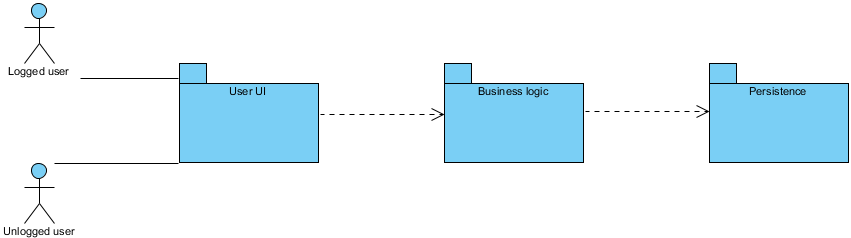
\includegraphics[width=\linewidth]{./images/basic-package}
\caption[Basic package]{Basic package diagram}
\label{fig:basic-package}
\end{figure}

\subsubsection{Detailed package design}
Given the functional requirements identified we can encapsulate them within specific components in the package diagram as follows:

\paragraph{User UI}
These set of sub packages are responsible for encapsulating the user actions and forwarding information requests to the Business logic sub packages.
\begin{itemize}
\item \emph{Login page:} this package implements FR2, FR5
\item \emph{Sign up page:} this package implements FR1
\item \emph{Calendar page:} this package implements FR3, FR7-FR12, FR14, FR15, FR19

\item \emph{Notification viewer:} this package implements FR13, FR16-FR18
\item \emph{User profile page:} this package implements FR4-FR6
\end{itemize}

\paragraph{Business logic}
These set of sub packages are responsible for handling requests from the User UI package, processing them and send back a response. These packages may access the Persistence package.
\begin{itemize}
\item \emph{Login manager:} this package implements FR2, FR3
\item \emph{User profile manager:} this package implements FR1, FR4-6
\item \emph{Calendar manager:} this package implements FR7-FR11, FR14, FR15
\item \emph{Search manager:} this package implements FR12, FR14, FR15
\item \emph{Notification manager:} this package implements FR13,FR16-FR19
\item \emph{Forecast manager:} this package implements FR17-FR19
\end{itemize}

\paragraph{Persistence}
This sub package contains the data model for the system. It accepts requests from the Business Logic package.
\begin{itemize}
\item \emph{Entity manager:} This package implements FR1-FR19
\end{itemize}

\begin{figure}[h!]
\centering
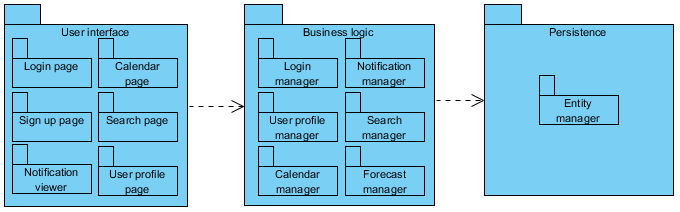
\includegraphics[width=\linewidth]{./images/detailed-package}
\caption[Detailed package]{Detailed package diagram}
\label{fig:detailed-package}
\end{figure}

\clearpage
\part{Design considerations}
This section encompasses the design considerations taken into account in the MeteoCal system design. Assumptions, dependencies, general constraints and performance requirements are clearly stated.

\section{Assumptions}
WHERE ARE THE ASSUMPTIONS??

\section{Dependencies}
\begin{tabular}{| p{0.3\linewidth} | p{0.7\linewidth} |}
\hline	\emph{Dependency}	&	\emph{Impact}	\\
\hline	Java virtual machine that supports JEE7 is already installed on the OS. & MeteoCal only runs on operating systems that support the JEE7 platform.	\\
\hline	The supported browsers will be Firefox and Chrome & MeteoCal outputs XHTML code that requires browsers that support most of the web standards, elsewhere the UI experience will be affected.	\\
\hline	A JEE7 AS is required on the server side	&	MeteoCal cannot operate if there is no AS that supports the JEE7 standard	\\
\hline
\end{tabular}

\section{General constraints}
This section describes the NFRs and the QoS details related to the design of the software product.

\noindent\begin{tabular}{| p{0.3\linewidth} | p{0.7\linewidth} |}
\hline	\emph{Element}	&	\emph{Requirement}	\\
\hline	Memory			&	2 GB+				\\
\hline	Database server	&	MySQL				\\
\hline	Network			&	Internet access, HTTP protocol	\\
\hline	Security		&	User data will be encrypted. SSL is not supported	\\
\hline	Hard disk space	&	40 GB+				\\
\hline
\end{tabular}


\clearpage
\part{Detailed software design}
\section{Database model}
\subsection{Conceptual Design}
We developed the entity-relationship diagram following what we specified in the class diagram presented in the RASD. 
\paragraph{Notes}
\begin{itemize}
\item In the future the possibility of changing the user name could be implemented. Therefore we used an integer ID as the User primary key instead of the user name.In this way it will be simpler to manage future changes in the way the system manages user data. 
Emails can already be changed and thus weren't a suitable choice for the primary key.
\item Places have an ID as primary key. It's the id that identifies the specified city in Open Weather Map (the external service used to get forecasts). In this way it will be simpler to manage places and forecasts according to the external service.   
\end{itemize}
\paragraph{ER diagram description}
The User entity contains all the  user's personal information. A user has exactly one calendar. A user can create events and he may receive notifications.\
Calendar is a weak entity with respect to User because if a user is deleted from the database's records then there's no need  to keep track of its calendar. A calendar contains 0 or more events.\
An event is created by exactly one user and it's contained in at least one calendar (the one belonging to its creator). Events can generate notifications. An event is held in one Place (that may be unspecified) and has a related forecast, if available.\
A Place is the location of at least one Event. It can also be the object of some weather forecasts.\
Forecast is a weak entity with respect to Place because forecasts referring to places that are not in the DataBase make no sense. A forecast has to be used by at least one event, otherwise it would be useless.\
A notification has to have at least one receiver and it concerns exactly one event. ECN, BWA, SDP and Invite are heir classes of Notification because they share the basic structure but have to be managed in different ways.



\clearpage
\tableofcontents
\end{document}